\documentclass[a4paper,11pt]{scrartcl}
\usepackage{helvet}
\renewcommand{\familydefault}{\sfdefault}


%% pacchetti 
%% ------------------------------------------------------------------------------------
\usepackage[T1]{fontenc}
\usepackage[utf8]{inputenc}
\usepackage[UKenglish]{babel}
\usepackage{lmodern, fancyhdr, lastpage, xspace, marvosym }
\usepackage[margin=25mm,
			%includehead
			]{geometry}
\usepackage{setspace}
\usepackage{lscape}
\usepackage{clipboard} %for copying text in several parts of the document






\usepackage[usenames,dvipsnames,table]{xcolor}
\usepackage{csquotes}
\usepackage[nohyperlinks,nolist]{acronym}

\usepackage{enumitem}

\usepackage{soul} % for smarter (word-wrapping) underlining.
\usepackage{tcolorbox}

\usepackage[textsize=9]{todonotes}
\newcommand{\todocd}[1]{{\textcolor{orange}{#1}}}
\newcommand{\todohost}[1]{{\textcolor{green}{#1}}}

%tables & pictures
%------------------------------------------------------------------------------------
\usepackage{multirow,bigdelim, caption, longtable} % longtable for tables that can fit on multiple pages
\captionsetup[longtable]{position=below} 
\usepackage{booktabs}
\usepackage{graphicx}

%% bibliography
%%--------------------------------------------------------------------------------

% usata con \nobibliography
\usepackage[ibidem, titleformat=commasep, lookat, citefull=first]{jurabib}
\renewcommand{\cite}{\footcite} % citations in footnotes




%% math
%%------------------------------------------------------------------------------------
\usepackage{amsfonts, amsmath, amsthm, amssymb, mathrsfs, amscd}		
\usepackage{xfrac}

%% hyperref e pacchetti fastidiosi
%%--------------------------------------------------------------------------------
\usepackage{xurl}
\usepackage[colorlinks = true,
            linkcolor = blue,
            urlcolor  = blue,
            citecolor = blue,
            anchorcolor = blue]{hyperref}


%% ridefinizioni e layout
%% -------------------------------------------------------------------------------
% \usepackage[subtle, mathdisplays=tight, lists=tight, bibnotes=tight, indent=tight,  
%% sections=tight,
%%charwidths=tight
%  ]{savetrees}
%  

%\headheight=14pt

%% Explicitly set footnote font size to match call (i.e., 8pt).
%% Taken from http://tex.stackexchange.com/a/249422/84485
\makeatletter
\renewcommand\footnotesize{%
	\@setfontsize\footnotesize\@ixpt{8}%
	\abovedisplayskip 8\p@ \@plus2\p@ \@minus4\p@
	\abovedisplayshortskip \z@ \@plus\p@
	\belowdisplayshortskip 4\p@ \@plus2\p@ \@minus2\p@
	\def\@listi{\leftmargin\leftmargini
		\topsep 4\p@ \@plus2\p@ \@minus2\p@
		\parsep 2\p@ \@plus\p@ \@minus\p@
		\itemsep \parsep}%
	\belowdisplayskip \abovedisplayskip
}
\makeatother







%% To correctly align fancy headers.
%% Courtesy of: http://tex.stackexchange.com/a/88136/84485
\makeatletter
\newcommand{\resetHeadWidth}{\fancy@setoffs}
\makeatother


\pagestyle{fancy}
\fancyhead{}
\fancyhead[R]{\color{gray}{Page \thepage~of \pageref*{sec:endpage}}}
\fancyhead[C]{\color{gray}{Tutor notes for small group teaching, \today}}
\fancyhead[L]{\color{gray}{Clinical studies}}
\cfoot{}



%%definizioni per mate
%%------------------------------------------------------------------------------------
\theoremstyle{plain}
\newtheorem{thm}{Theorem}[section]

\theoremstyle{remark}
\newtheorem{rmk}[thm]{Remark}
\newtheorem{propy}[thm]{Property}
\newtheorem{step}[thm]{Step}

\theoremstyle{definition}
\newtheorem{defn}[thm]{Definition}
\newtheorem{exam}[thm]{Example}
\newtheorem{note}[thm]{Note}
\newtheorem{quest}[thm]{Question}



%%tikz stuff 
%%-----------------------------------------------------------------------------------
\usetikzlibrary{positioning,calc} 
\tikzset{shifted by/.style={to path={($(\tikztostart)!#1!90:(\tikztotarget)$)
 -- ($(\tikztotarget)!#1!-90:(\tikztostart)$)}}, 
 shifted by/.default=2pt,standard edge/.style={very thick,-latex}, 
 back and forth between/.style args={#1 and #2}{insert path={
  #1 edge[standard edge,-latex,shifted by] #2 #2 edge[standard edge,shifted by] #1}}} 
  
  
  
%% global settings
%%-----------------------------------------------------------------------------------


\title{TUTORS NOTES FOR SMALL GROUP TEACHING \\ Designing a clinical study for pancreatic cancer risk factors}
\date{}


%%-----------------------------------------------------------------------------------
%% begin document
%%-----------------------------------------------------------------------------------

\begin{document}
\begin{center}
{\LARGE DESIGNING A CLINICAL STUDY FOR PANCREATIC CANCER RISK FACTORS \\ \medskip Tutor notes for small group teaching}
\end{center}


%% In the following: instructions for the tutor. Note that
%% what is written in \Copy{scenario}{ - } is authomatically repeated
%% in the students' materials
%%-----------------------------------------------------------------------------------

\section{Introduction}
\label{sec:introduction}

The purpose of this activity is to give students the opportunity to think about the issues involved in designing case-control and cohort studies (future development: think about adding a cross-sectional study and a randomised control trial). The activity is designed to be used both for face-to-face teaching and for distant learners, with the due adaptations. A sheet will be handed out with the scenario and the scheme here included, and another, pre-filled with answers will be made available at the end of the activity. 

   
\section{Presentation (5 minutes)}

\textit{\textbf{Don't hand out sheets yet. }}

\medskip

With the use of a presentation, recap case-control and cohort studies designs, what is a biobank. Then move to the questions here below. 


\section{Setting the scenario (5-10 minutes)}

\textit{\textbf{Have a summary on the presentation and read out the following. This text will also be on the sheets that students will be handed later. }}
\medskip

\Copy{scenario}{Pancreatic cancer is the 10th most common cancer with 10,449 people diagnosed with pancreatic cancer in the UK in 2018. It has the lowest survival of all common cancers, with five-year survival less than 7\%. 

\medskip

Early diagnosis is crucial to improve survival outcomes, with one-year survival in those diagnosed at an early stage six times higher than one-year survival in those diagnosed at stage four.  
However, most people with pancreatic cancer are diagnosed at a late stage (UK statistics on \url{https://www.pancreaticcancer.org.uk/}). 
\medskip

Patients usually experience no specific symptoms until the cancer is in a late stage. Currently there is no screening programme for pancreatic cancer in the UK, nor are there data to show reduced mortality from pancreatic cancer from any screening test. The diagnosis is usually made by imaging, after late symptoms such as jaundice and weight loss have already developed. Some data provide preliminary support for use of imaging methods (endoscopic ultrasound and MRI) if patients screened are \textbf{at increased risk} of pancreatic cancer. Therefore an accurate, non-invasive way to identify people at sufficiently high risk could enable the development of pancreatic cancer screening. 

\medskip

Known risk factors for pancreatic cancers include age, sex, smoking, high body mass index (BMI), diabetes, certain chemicals, ethnicity, and family history. There have also been investigations on the utility of a variety of \textbf{biomarkers} to identify those at sufficiently increased risk of pancreatic cancer to justify screening using imaging.

\medskip
Cohort studies have a long history, but a recent development has been the use of biobanks from large population cohorts (such as UK Biobank - \url{https://www.ukbiobank.ac.uk}), that record data on participants from traditional questionnaires, in addition to biological samples, for instance to help evaluate the association between genetic variation, environmental exposures for risk of disease. Disease-specific biobanks have also been developed. One such at Barts Cancer Institute is the Pancreatic Cancer Research Fund Tissue Bank (PCRF, for further details see \url{https://www.thepancreastissuebank.org}). Set up in 2016, it has collected:
\begin{itemize}
\item Blood samples from 2,200 consenting patients who underwent biopsies or surgery for pancreatic diseases, including pancreatic cancers (also urine, saliva and tissue samples);
\item Large numbers of healthy control blood (also urine and saliva).
\end{itemize}
}


\subsection{Open questions}
\textit{\textbf{Ask, and take notes of answers on the whiteboard:}}

\begin{quest} ``How would you design a study to investigate whether or not a proposed biomarker (or a combined panel of biomarkers) is an effective tool for identifying those at high risk of pancreatic cancer, in order to enable early detection of pancreatic cancer?'' 
\end{quest}


\begin{itshape}
Hopefully students will get to (after prompting if necessary):
\begin{itemize}
	\item \textbf{Cross-sectional} study: take biological samples, evaluate the biomarker (or panel) at the same point in time as a diagnostic test for pancreatic cancer. For instance, run the study in those attending a GP appointment, or better, target a high risk group – eg. If registry people with strong family history for pancreatic cancer, or patients with diabetes mellitus. Would be difficult to run - no long term outcome; and pancreatic cancer is very rare so study would have to be enormous to find even a handful of cases.
\item Could do a \textbf{case-control} study to assess the performance of the biomarker in detecting pancreatic cancers across all stages. Any of the following might be discussed (don’t need to go through them all if not though) 
	\begin{itemize}
	\item Collect samples from patients with a new diagnosis of pancreatic cancer (blood and tissue) and select healthy controls without a diagnosis of cancer (blood). Think about who controls will be recruited and how.
	\item Use a biobank focused on pancreatic cancer for selecting participants with cancer, and controls without cancer from the same biobank (e.g. the Pancreatic Cancer Research Fund Tissue mentioned above \url{https://www.thepancreastissuebank.org}; controls might have benign ). Or use a cohort or trial from a population without pancreatic cancer at entry (e.g. UK Biobank~\url{https://www.ukbiobank.ac.uk}) where healthy patients are recruited and followed up, with bioloigical samples stored in a biobank. Here one might also do a \textbf{nested case-control} study by taking cases diagnosed within a certain time of entry, and matched controls, and use the biobank samples to run the tests. Suggest that we are working under the assumption that technology works on the available material and that storage does not degrade samples. 
	\end{itemize}
\item Do a \textbf{cohort} study to validate the use of the test in detecting pancreatic cancers earlier. Remark that the number of participants would be huge for a general population sample (eg. young), so likely need to enrich by recruiting a higher-risk group using other factors (e.g. diabetes mellitus, strong family history, ...). Think about possible ethical issues.
\item Could do a \textbf{randomised controlled trial}, where we use the biomarker to take some sort of action (screening with imaging, clinical work-up), but also here one must be careful of ethical issues (e.g. participants whose tests detects potential signals of cancer, or identified at very high risk, will need to be told their group and be referred for further tests. Would need evidence that the test does identify high risk before being used to take clinical actions).
\end{itemize}
\end{itshape}

\begin{note}
If students identify cohort and case-control studies as \textbf{prospective} and \textbf{retrospective} studies, try and discourage these terms. Cohort and case-control are more accurate, especially as you can do a prospective case-control study (nested case-control – where at the study's end, the cases and controls are sampled from a cohort) and you can do a retrospective cohort study where you collect a cohort from historical data.
\end{note}

\textit{\textbf{Ask, and take notes of answers on the whiteboard:}}

\begin{quest} ``What summary measure of risk associated with the biomarker could you use for each study?''
\end{quest}

\begin{itshape}
Classical metrics:
\begin{itemize}
\item Cohort study: relative risk – for example risk of pancreatic cancer in people who were biomarker positive divided by risk  in people who were biomarker negative, if binary. If continuous: relative risk per unit of the biomarker, or per SD of the biomarker. Also could consider a hazard or rate ratio, where the time-to-event is considered (where the event can be the diagnosis).
\item Case-control study:  odds ratio (again could be binary or continuous per unit etc).
\end{itemize}

Metrics for diagnostic tests (not covered in preliminary material, but if raised good to discuss):
\begin{itemize}
\item Sensitivity: the proportion of test-positive subjects out of all disease-positive subjects. Independent of prevalence.
\item Specificity: proportion of test-negative subjects out of all disease-negative subjects. Independent of prevalence.
\item Positive Predictive Values (PPV): probability that following a positive test result, that individual will truly have that specific disease. Depends on prevalence. 
\item Negative Predictive Values (NPV): probability that following a negative test result, that individual will truly not have that specific disease. Depends on prevalence. 
\end{itemize}

	\textbf{Summary:} either take people without disease, evaluate the biomarker and follow them up to assess risk in each group, hence RR or HR; or take people with disease and without disease, and assess the biomarker (odds ratio). Remark that OR is equivalent to RR and HR it the disease is rare.

\end{itshape}
\section{Group activity}

\subsection{Work in small groups (30 minutes)}

\textit{\textbf{Split the students into (muliples of) two groups (no more than 8 in each group) and tell them:}}

\medskip

\Copy{TheQuestion}{``Assume that Cancer Research UK is going to fund two different studies to investigate whether your research group’s biomarker panel can help stratify risk of pancreatic cancer, and enable early detection that might lead to improvements in public health outcomes. One will be a case-control study, that will report its results within 3 years and the second group they need to design a cohort study which will report its results within 13 years.''}

\medskip


\begin{description}
\item[Group A (and multiples)] needs to design a case-control study that reports results within 3 years;
\item[Group B] design a cohort study that reports results within 13 years.
\end{description}


\textit{\textbf{Hand out the student sheets which contain the questions to fill in to design the studies (the first group should answer the left hand column and the second group the right hand column).}}



\subsection{Group presentations (25 minutes)}


%%-----------------------------------------------------
%% Students materials 
%%-----------------------------------------------------


\begin{landscape}
\section{Annotated students' materials}
\subsection{Cohort and case control studies and possible metrics}

%changing font size for the students materials to be clearer
\begin{large}

\begin{center}
\LARGE{Cohort study}
\end{center}

\begin{center}
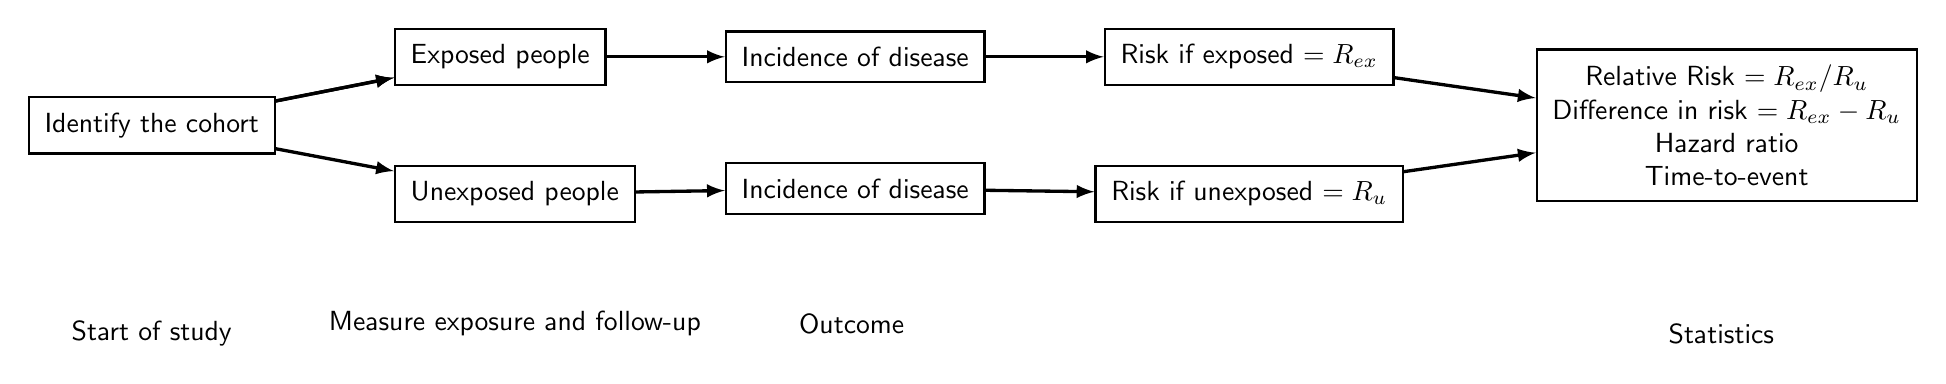
\begin{tikzpicture}[boot/.style={draw,thick,align=center, inner sep=2mm}]
\node[boot=20] (CH) {Identify the cohort};
\node[above right=0.5cm and 1.5cm of CH.east,boot=20] (EP) {Exposed people};
\node[below right=0.5cm and 1.5cm of CH.east,boot=20] (UP) {Unexposed people};
\node[right=1.5cm of EP,boot=20] (ID1) {Incidence of disease};
\node[right=1.5cm of UP, below=1cm of ID1, boot=20] (ID2) {Incidence of disease};
\node[right=1.5cm of ID1,boot=20] (RE) {Risk if exposed $= R_{ex}$};
\node[right=1.5cm of ID2, below=1cm of RE, boot=20] (RU) {Risk if unexposed $= R_{u}$};
\node[right=16cm of CH,boot=20] (STAT) {Relative Risk $= R_{ex} / R_{u}$ \\ Difference in risk $= R_{ex} - R_{u}$ \\ Hazard ratio \\ Time-to-event};

\node[below=2cm of CH,align=center] (SS) {Start of study};
\node[right=1cm of SS, below=1cm of UP,align=center] (ME) {Measure exposure and follow-up};
\node[right = 1cm of ME, align=center] (OC) {Outcome};
\node[right=18cm of SS,align=center] (STATD) {Statistics};

\draw (CH) edge[standard edge] (EP)
(CH) edge[standard edge] (UP)
(CH) edge[standard edge] (EP)
(EP) edge[standard edge] (ID1)
(UP) edge[standard edge] (ID2)
(ID1) edge[standard edge] (RE)
(ID2) edge[standard edge] (RU)
(RE) edge[standard edge] (STAT)
(RU) edge[standard edge] (STAT)

;
\end{tikzpicture}
\end{center}




\begin{center}
\LARGE{Case-control study}
\end{center}

\begin{center}
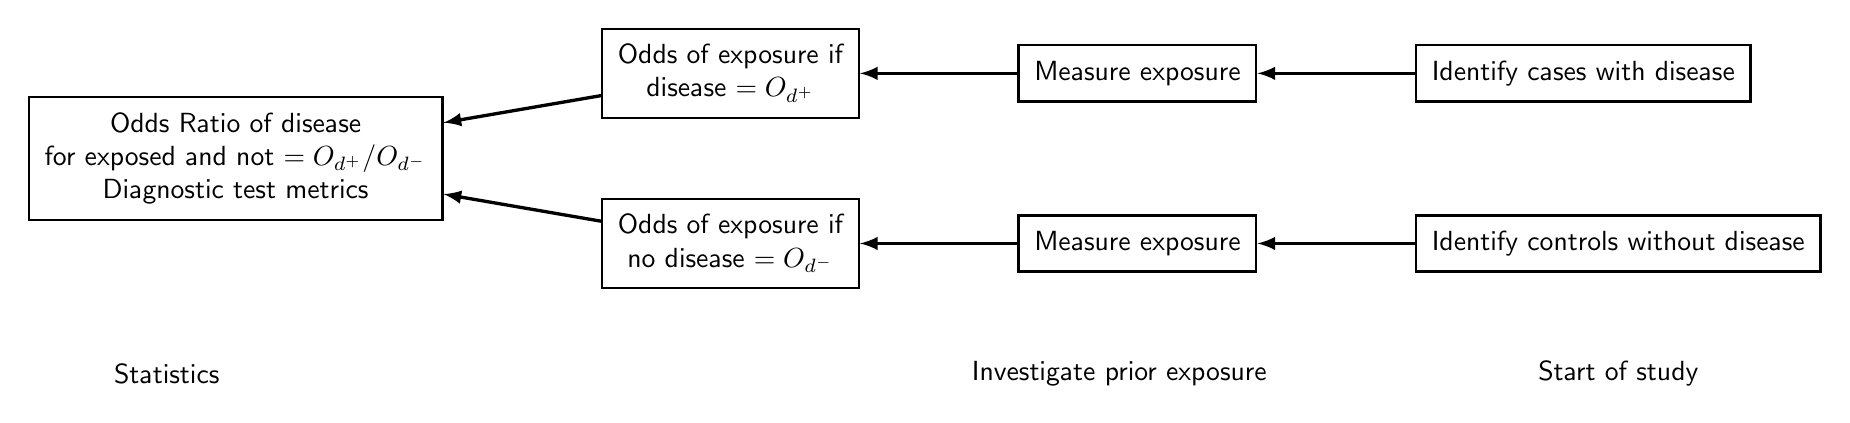
\begin{tikzpicture}[boot/.style={draw,thick,align=center, inner sep=2mm}]

\node[boot=20] (STAT) {Odds Ratio of disease \\  for exposed and not $ = O_{d^+}/ O_{d^-}$\\ Diagnostic test metrics };
\node[above right=0.5cm and 2cm of STAT.east,boot=20] (OD) {Odds of exposure if \\ disease $=O_{d^+}$};
\node[below right=0.5cm and 2cm of STAT.east,boot=20] (OND) {Odds of exposure if \\ no disease $=O_{d^-}$};
\node[right=2cm of OD,boot=20] (ME1) {Measure exposure};
\node[right=2cm of OND, boot=20] (ME2) {Measure exposure};
\node[right=2cm of ME1,boot=20, anchor=west] (ICa) {Identify cases with disease};
\node[right=2cm of ME2, boot=20, anchor=west] (ICo) {Identify controls without disease};



\node[below=1cm of ICo,align=center] (SS) {Start of study};
\node[left=3.2cm of SS, align=center] (IPE) {Investigate prior exposure};
\node[left=16.5cm of SS,align=center] (STATD) {Statistics};

\draw (ICa) edge[standard edge] (ME1)
(ICo) edge[standard edge] (ME2)
(ME1) edge[standard edge] (OD)
(ME2) edge[standard edge] (OND)
(OD) edge[standard edge] (STAT)
(OND) edge[standard edge] (STAT);
\end{tikzpicture}
\end{center}




\clearpage

\Paste{scenario}

\bigskip

\Paste{TheQuestion}

\bigskip

In answering the question you will need to think about the following. 


\clearpage

\begin{longtable}{p{0.45\linewidth} | p{0.45\linewidth}  }
%% Title row -------------------------------
\toprule
\textbf{A: Case-control study with results in 3 years} &\textbf{B: Cohort study with results in 13 years} \\ 
\toprule

%% First question -------------------------------
{\raggedright{{What are your entry criteria for \textbf{cases}?

\bigskip

\textit{They have to have pancreatic cancer. Think if they'd better be newly diagnosed, anyone with it (and at which stage?), or those that have died (most people with pancreatic cancer die from it). }}}} 
&
\multirow{3}{=}{
\raggedright{What characteristics of the cohort will make the follow up easier and enable you to obtain useful results? Think about who will you recruit - what type of people, for where and how, how many

\bigskip


\textit{- People who are easy to keep track of (so helpful to have some method of finding them if leave work) and likely to be motivated to fill forms in and come back for check-ups.
\newline
It needs to be large enough so that enough will get the disease in the next 13 years and/or is at high risk from other factors.
\newline
- They need to be old enough / high risk enough so that enough will get the disease in the next 13 years and not too old because they may be quite likely to die of something else in next 15 years, so probably something like 50-79 years old. 
\newline
- They need to come from backgrounds and ethnicities representative of the target population.}
}}
\\

\cmidrule{1-1} & \\
%% Second question -------------------------------
\raggedright{Most case-control studies match cases and controls. What would you match on and what are your entry criteria for \textbf{controls}?

\bigskip

\textit{Entry criteria for controls - don't have the disease (if they did they should be a case), with no known diagnosis or past history of pancreatic cancer.
\newline
Get a control for each case (or other reasonable ratio). 
\newline
	Controls should be matched to achieve balance in important demographic characteristics (age, gender), to increase efficiency of estimation (eg. if you want to compare the utility of the biomarker in people older than 70y you need to have controls >70y, matching would ensure this)
\newline
Remember that matching on too many things will make it difficult and overmatching can lead to cases and controls not differing enough in the exposure
}
}& \\
\cmidrule{1-1} & \\
%% Third question -------------------------------
\raggedright{Describe how you will recruit to the case control study (remember you can use a biobank)

\bigskip

\textit{Retrospectively collected samples from a biobank (controls can be either healthy individual registered in the biobank, or individuals who are registered in the biobank as subjects with various diseases that are not pancreatic cancer).
\newline
	Or (prospective) consent new patients with pancreatic cancer from hospital (cases), and controls in the same hospitals, or at least geographical region from where the cases were recruited, or healthy volunteers, blood donors, \ldots 
}
}& \\
\midrule
%% Forth question -------------------------------
\multicolumn{2}{c}{What is a simple binary risk factor or exposure?} \\ 
{\raggedright{

\bigskip 
\textit{Biomarker positive/negative at diagnosis\footnote{Ideally biomarker positivity is pre-defined, perhaps based on a cutpoint if the underlying biomarker is a continuous variable.}.}}}
&
{\raggedright{

\bigskip 
\textit{Biomarker positive/negative prior to diagnosis\footnote{as before.}.}}}
\\
\midrule
%% Question -------------------------------
\multicolumn{2}{c}{How else could you measure the risk factor (biomarker)?} \\ 
\multicolumn{2}{p{0.9\linewidth}} 
{\raggedright{

\bigskip 
\textit{The biomarker might be a continuous variable, not binary. For example, gene expression could be categorised as high vs low, or the raw intensity used as a biomarker. Using a continuous variable is almost always more informative than a categorical version of the same marker.}}} \\
\midrule
%% Question -------------------------------
\multicolumn{2}{c}{Briefly describe how you would determine the value of biomarker and other risk factors.} \\ 
{\raggedright{

\bigskip 
\textit{Testing samples previously stored in the biobank. Questionnaires for classical risk factors.}}}
 & 
{\raggedright{

\bigskip 
\textit{Test samples on everyone at entry, and potentially also through time (additional samples and questionnaires).}}}
\\
\pagebreak
\midrule
%% Question -------------------------------
\multicolumn{2}{c}{Give the single most accurate and useful simple binary measure of outcome for your study.} \\ 
{\raggedright{

\bigskip 
\textit{Pancreatic cancer}}}
&
{\raggedright{

\bigskip 
\textit{Death from pancreatic cancer or diagnosis of pancreatic cancer - because pancreatic cancer has such a poor prognosis there is little difference. Death from cancer may be a better outcome for tracking, because even if someone is lost to follow-up we can usually still find out if they have died and from what cause using death certificates. For other cancers, death from the cancer may be a stronger outcome than disease incidence because of overdiagnosis (but not covered in this course).}}} \\
\midrule
%% Question -------------------------------
\multicolumn{2}{c}{Who will the actual results be representative of?} \\ 
{\raggedright{

\bigskip 
\textit{If the case-control study is well designed, it would be representative of the study population that cases and controls are supposed to have arisen from - from where the cases and controls came.}}}
& 
{\raggedright{

\bigskip 
\textit{The social and demographic make up of members of the cohort.}}} \\
\midrule
%% Question -------------------------------
\multicolumn{2}{c}{Who will these results be useful for?} \\ 
\multicolumn{2}{p{0.9\linewidth}}
{\raggedright{

\bigskip
\textit{Because RR/HR and OR are generally robust to different populations - to everyone who might benefit of a screening program, so eventually for everyone. }}} \\
\midrule
%% Question -------------------------------
\multicolumn{2}{c}{What other results could your get from your study group?} \\
{\raggedright{

\bigskip 
\textit{Could search for other different risk factors to see if associated with pancreatic cancer.}}}
&
{\raggedright{

\bigskip
\textit{Could ask or test about different risk factors to see if associated with pancreatic cancer and could follow up for different types of cancer or causes of death}}}
\\
\pagebreak
\midrule
%% Question----------------------------------
\multicolumn{2}{c}{Could the age of the participants affect the interpretation of your results?  If so how?} \\ 
{\raggedright{

\bigskip
\textit{No because you have matched for age.}}} 
&
{\raggedright{

\bigskip
\textit{Yes, if age is correlated with the biomarker, but the biomarker does not add information beyond age (age is a confounding factor). For this reason one would like to adjust for age in the analysis.}}}
\\
\midrule
\multicolumn{2}{c}{What biases could occur from your study design?} \\ 
\raggedright{
\bigskip

\textit{Main bias is inappropriate controls - selection bias. For instance, if controls are selected for inclusion using a criteria that is linked (correlated) with the biomarker. 
\newline
Confounding for other risk factors
\newline
Participants with cancer were not detected at an early stage - not asymptomatic; to understand performance for early detection would ideally have a sample from cases prior to diagnosis. Will require additional studies.
}}& 
{
\raggedright{
\bigskip

\textit{Not many - those in the cohort may be a selected (self or otherwise group) but the effect of having a biomarker or not is unlikely to be different in them than in those who were not asked or declined to take part. Bias may occur due to loss to follow-up but obtaining death certificates would overcome this.}}}
\\
\midrule
%% Question ------------------------------------
\multicolumn{2}{p{0.9\linewidth}}
{\centering Give an example of a study of an exposure and a disease that would be unsuitable for your type of study but suitable for the other.\newline Explain the characteristics of the exposure or disease that make it unsuitable} \\ 
{\raggedright{
\bigskip

\textit{A rare exposure that is associated with the disease but not the main cause of it. Would be unlikely to get anyone in the case control with the exposure.}}} & 
{\raggedright
\bigskip

{\textit{Rare diseases - even if you have a large cohort it is unlikely that enough people can be followed up. }}}\\
\midrule
%% Question ---------------------------------
\multicolumn{2}{c}{Summarise the advantages in general of your type of study?} \\ 
{\raggedright
\bigskip

{\textit{Cheaper than cohort.
\newline
Relatively quick.
\newline
Good for rare diseases.
}}}&
{\raggedright
\bigskip

{\textit{Generally less biased than case control studies. 
\newline
Can estimate risks and difference in risks as well as relative risks.
\newline
Can look at more than one outcome.}}}
 \\
\pagebreak
\midrule
%% Question ------------------------------
\multicolumn{2}{c}{Summarise the disadvantages in general of your type of study?} \\ 
{\raggedright
\bigskip

{\textit{
Can't do for rare exposures
Suffers from confounding (other than  the variables matched on)
In general, selection bias
Possible poor controls. 
}} }
&
{\raggedright
\bigskip

{\textit{
It is time consuming and expensive. 
\newline
Suffers from confounding.
}}}
 \\
\bottomrule 
\caption{Fill in the side corresponding to your group.}
\label{T:twostudies}
\end{longtable}
 
Further reading:
\begin{itemize}
\item Early detection of pancreatic cancer: \url{https://pubmed.ncbi.nlm.nih.gov/32135127/}
\item Description of the UROPANC trial: \url{https://www.bartscancer.london/centre-for-experimental-cancer-medicine/clinical-trial-portfolio/uropanc/}
\item A combination of urinary biomarker panel and PancRISK score for earlier detection of pancreatic cancer: A case–control study: \url{https://www.ncbi.nlm.nih.gov/pmc/articles/PMC7758047/}
\item Germline BRCA2 K3326X and CHEK2 I157T mutations increase risk for sporadic pancreatic ductal adenocarcinoma: \url{https://onlinelibrary.wiley.com/doi/10.1002/ijc.32127}
\item Noninvasive Diagnosis of Pancreatic Cancer Through Detection of Volatile Organic Compounds in Urine: \url{https://pubmed.ncbi.nlm.nih.gov/29129714/}
\item Biomarkers in molecular medicine: cancer detection and diagnosis: \url{https://www.future-science.com/doi/10.2144/05384SU04}
\item Empirical Evidence of Design-Related Bias in Studies of Diagnostic Tests: \url{https://jamanetwork.com/journals/jama/fullarticle/191668}
\item Statistical Hypothesis Testing versus Machine Learning Binary Classification: Distinctions and Guidelines: \url{https://www.sciencedirect.com/science/article/pii/S2666389920301562}
\end{itemize}



\end{large}
\label{sec:endpage}
\end{landscape}
\end{document}
